\section{電源系 (概要/EPS/インヒビット設計(二重絶縁)/電源系統図/電池/SAP)(池谷・中塚)}
\subsection{概要}
本節では本衛星の電源系について述べる.

本衛星の電源系の概要を

に示す.

電源系統図挿入

本衛星の電源系は主に以下のコンポーネントから構成されている.
\begin{itemize}
	\item 太陽電池パネル(Solar Array Panel, SAP)
	\item 電源基板EPS
	\item バッテリ
	\item インヒビット回路
	\item CIB電源系
	\item 伸展カメラ部電源系
\end{itemize}


\begin{landscape}
\begin{figure}[htbp]
	\begin{center}
		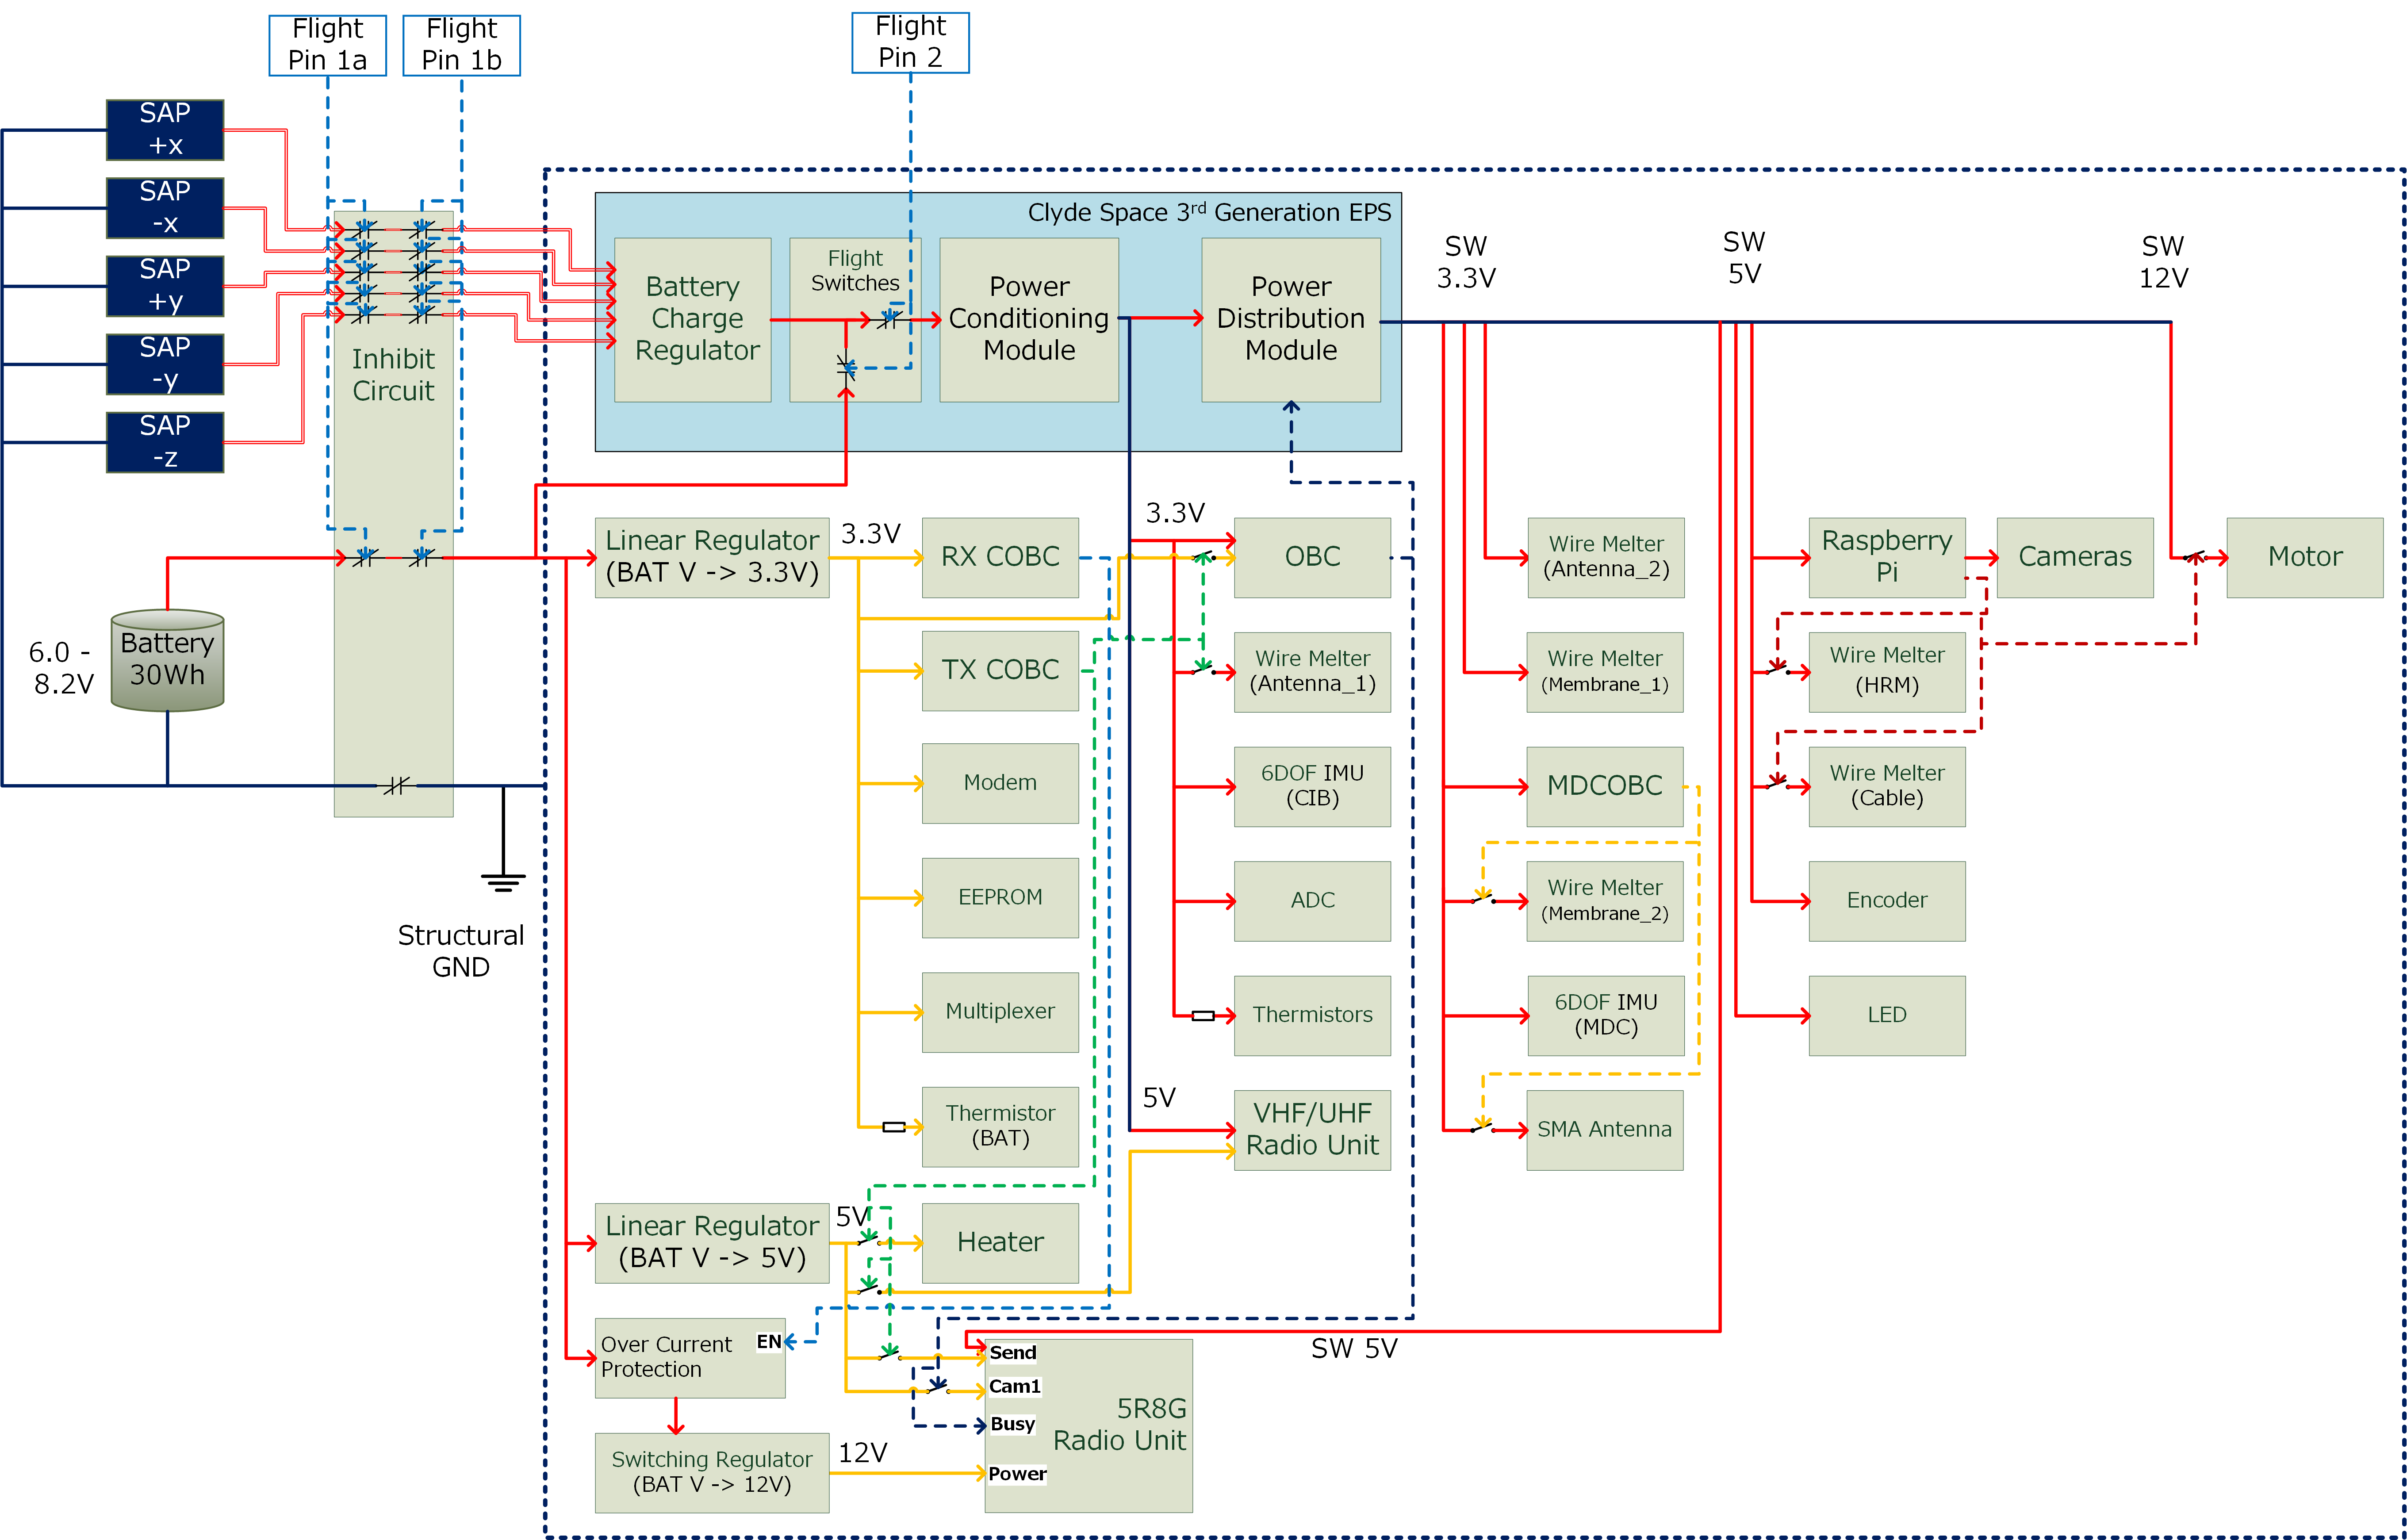
\includegraphics[width=0.5\linewidth]{./03/fig/Power_diagram.png}
		\caption{Example of a figure caption.}
		\label{power_diagram}
	\end{center}
\end{figure}
\end{landscape}            


\subsection{SAP}

\subsubsection{SAP試験}

\subsection{バッテリ}
バッテリはClyde Space社の30Whr Standalone CubeSat Batteryを購入した
図
.バッテリの諸元を表

に示す

また絶対最大定格を

に示す.

\begin{figure}[htbp]
	\begin{center}
		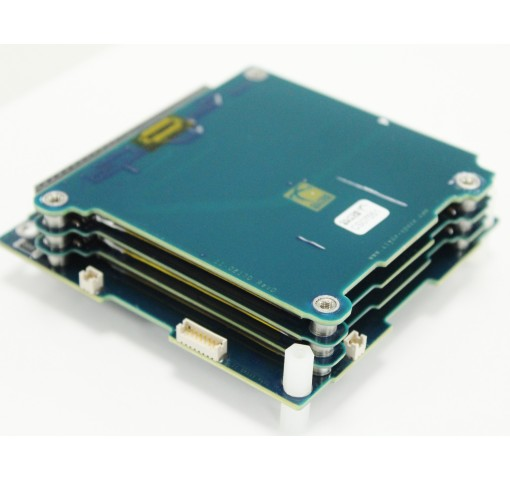
\includegraphics[width=0.5\linewidth]{./03/fig/battery.jpg}
		\caption{30Whr Standalone CubeSat Battery (c)Clyde Space}
		\label{mir}
	\end{center}
\end{figure}

\begin{table}[htbp]
	\begin{center}
		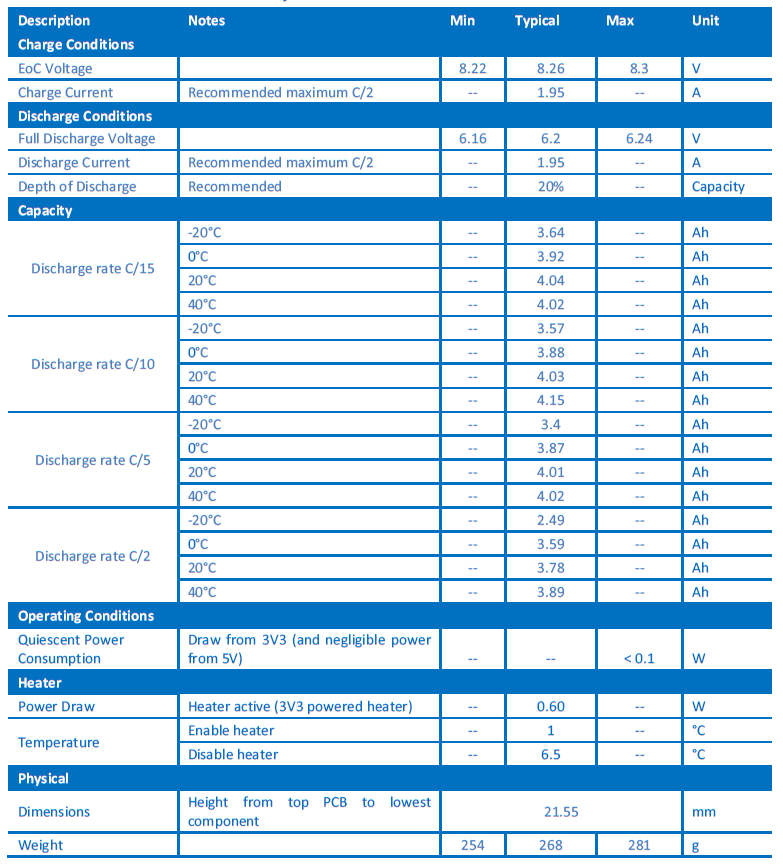
\includegraphics[width=0.8\linewidth]{./03/fig/battery_spec.png}
		\caption{30Whr}
		\label{mir}
	\end{center}
\end{table}

絶対最大定格

本バッテリは内部保護機能

\begin{figure}[htbp]
	\begin{center}
		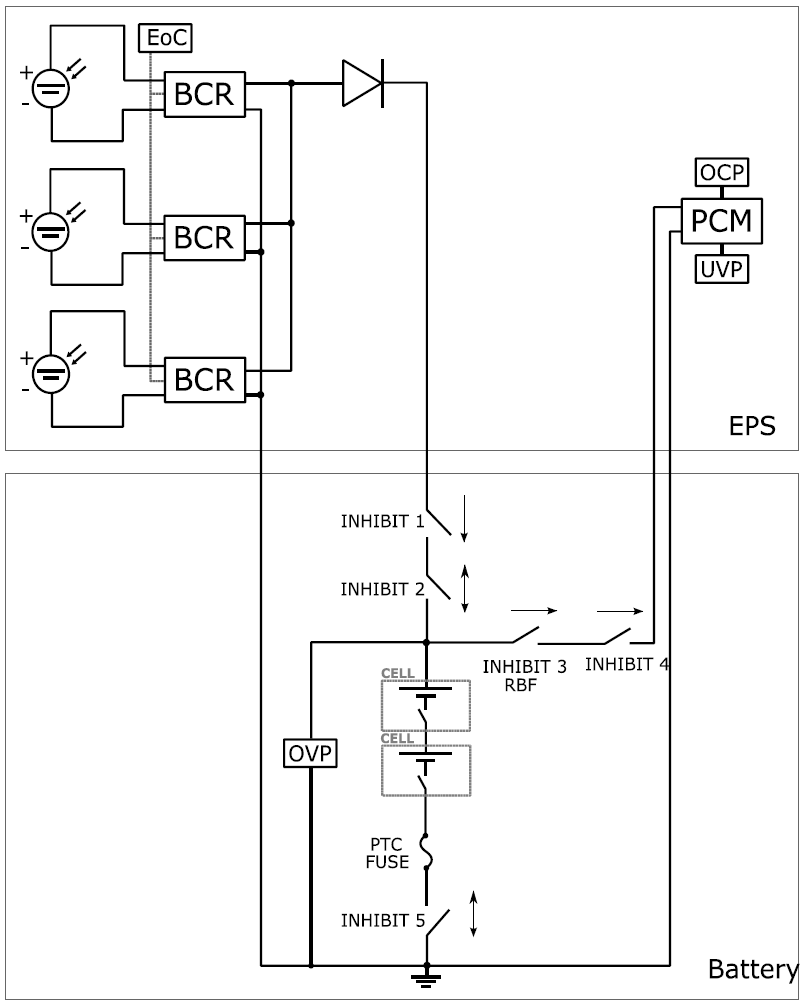
\includegraphics[width=0.5\linewidth]{./03/fig/bat_protection.png}
		\caption{Integrated EPS and Battery Protection Architecture 転載}
		\label{mir}
	\end{center}
\end{figure}

\begin{figure}[htbp]
	\begin{center}
		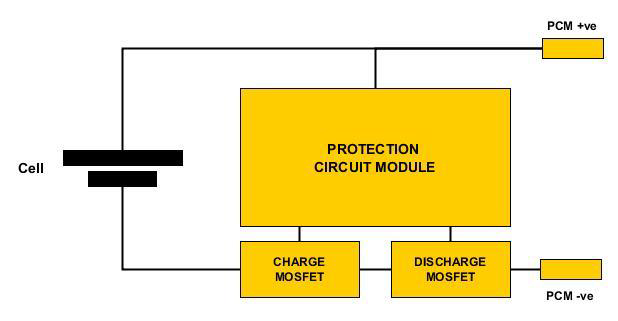
\includegraphics[width=0.5\linewidth]{./03/fig/cell_protection.png}
		\caption{Integrated EPS and Battery Protection Architecture 転載}
		\label{cell_p}
	\end{center}
\end{figure}


\subsection{CIB電源系}

\begin{figure}[htbp]
	\begin{minipage}{0.5\hsize}
		\begin{center}
			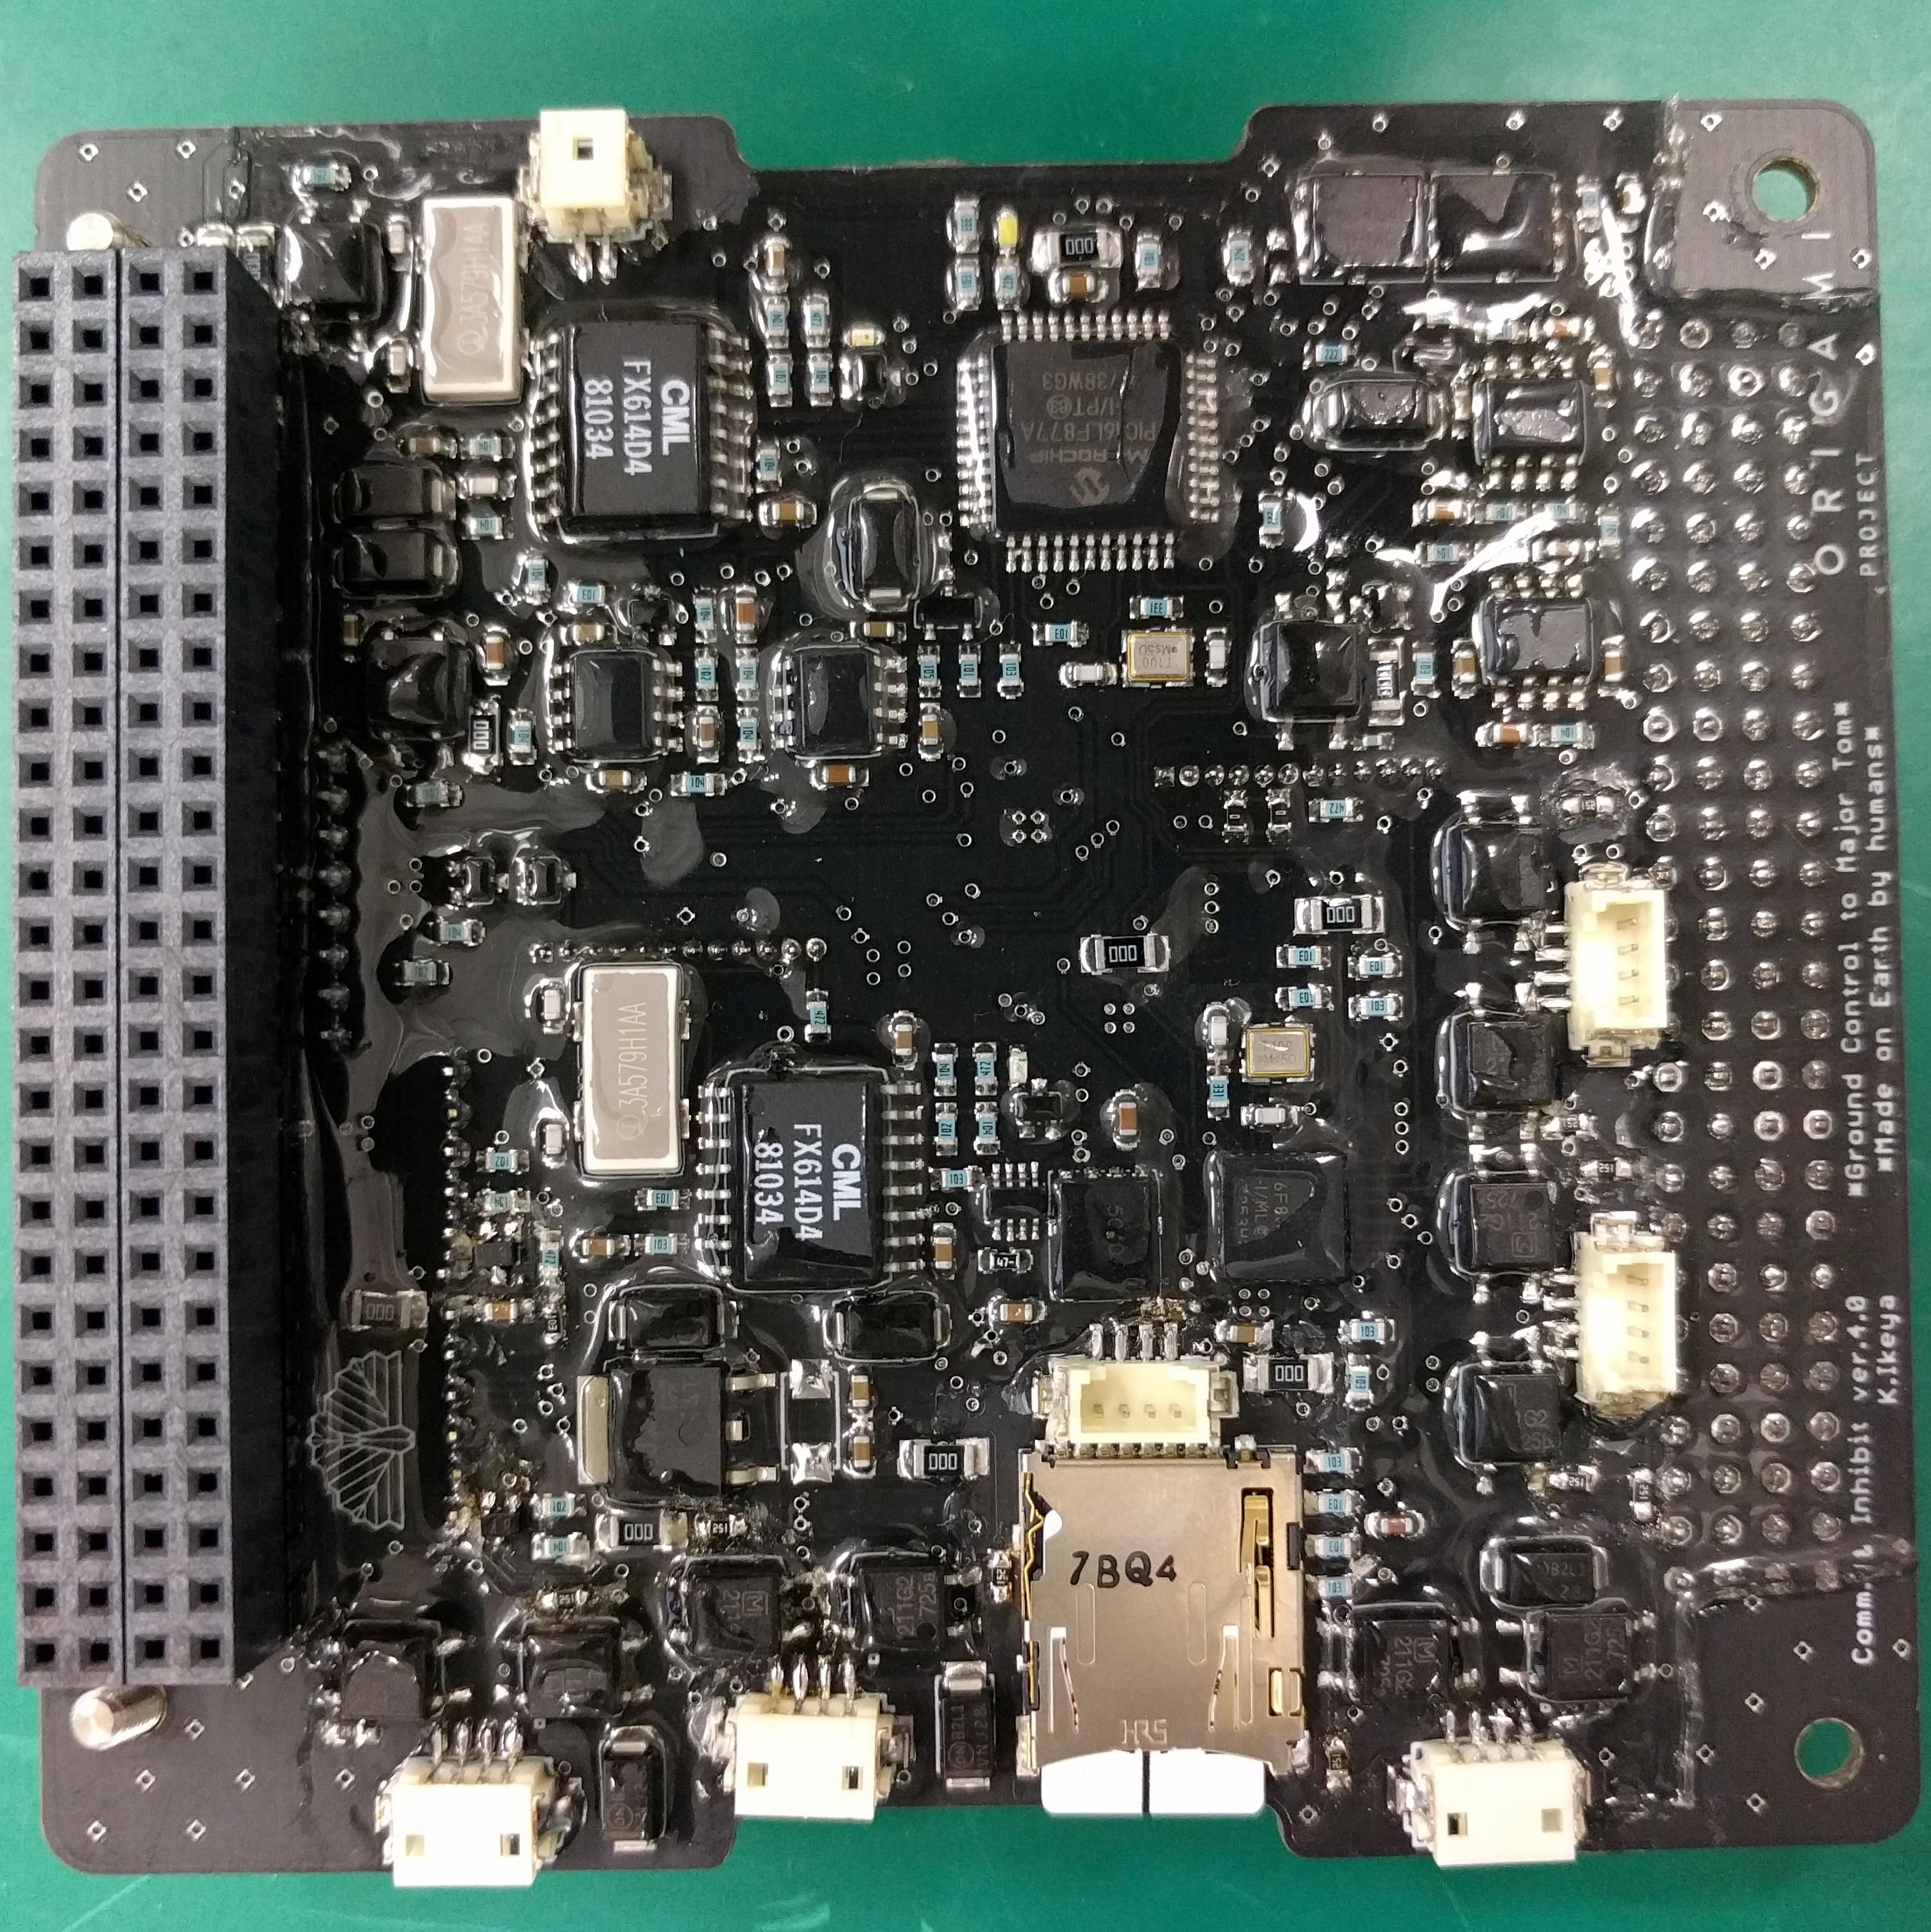
\includegraphics[width=0.7
			\linewidth]{./03/fig/CIB_1.jpg}
		\end{center}
	\end{minipage}
	\begin{minipage}{0.5\hsize}
		\begin{center}
			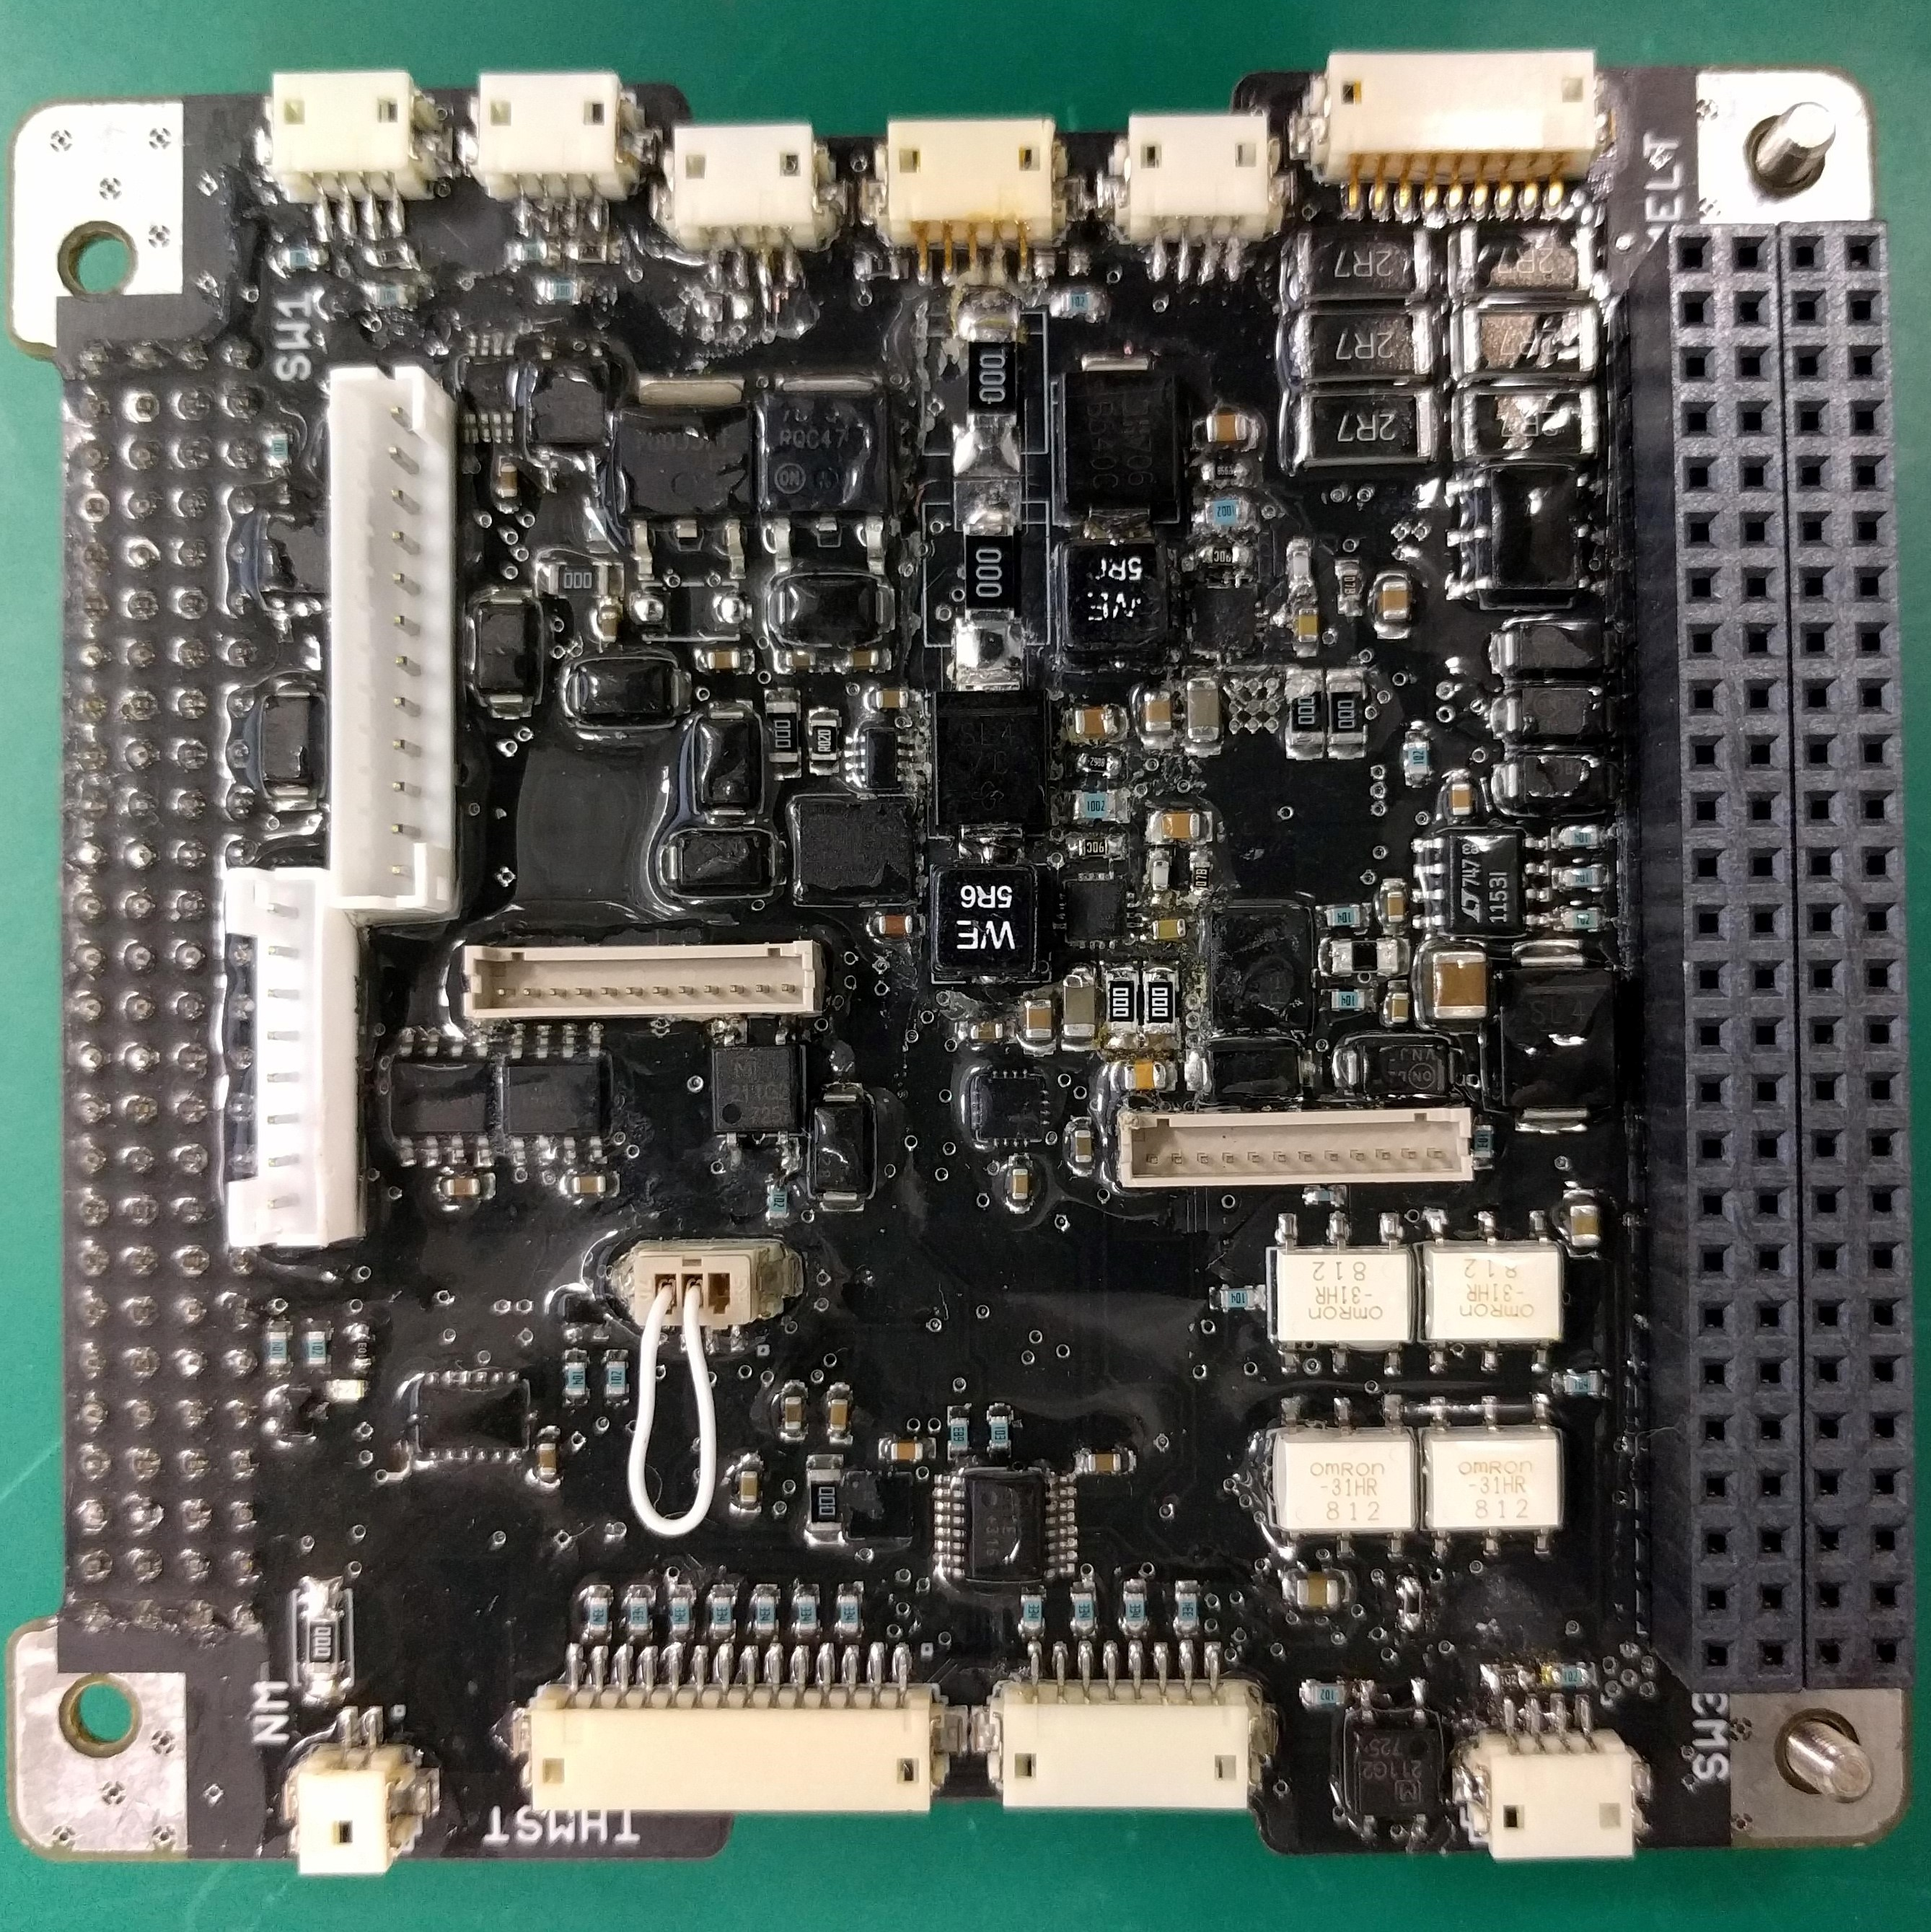
\includegraphics[width=0.7\linewidth]{./03/fig/CIB_2.jpg}
		\end{center}
	\end{minipage}\\		
	\begin{center}
		\caption{CIB}
	\end{center}
\label{CIB}
\end{figure}

\subsubsection{インヒビット回路}


\subsubsection{電源回路}
RXCOBCおよびTXCOBCは
UHF/VHF無線機
はほとんどの場合起動していないければならない

そこで新たな電源回路を設けた



\subsection{EPS}
EPSは

を購入した
\begin{figure}[htbp]
	\begin{center}
		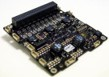
\includegraphics[width=0.5\linewidth]{./03/fig/eps.png}
		\caption{EPS}
		\label{eps}
	\end{center}
\end{figure}

\subsection{ミッション部電源系}
ミッション部電源系は
Raspberry Pi
が受け取ったUART信号により
スイッチのON/OFFを切り替える
\ref{}にて
後述する


